\vspace{2mm}
\begin{figure}[h!]
\tikzset{every picture/.style={line width=0.75pt}} %set default line width to 0.75pt        

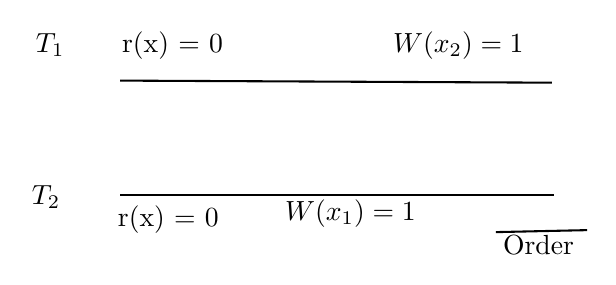
\begin{tikzpicture}[x=0.75pt,y=0.75pt,yscale=-1,xscale=1]
%uncomment if require: \path (0,300); %set diagram left start at 0, and has height of 300

%Straight Lines [id:da9500410641573396] 
\draw    (63.56,64) -- (271.56,65) ;
%Straight Lines [id:da7796185686481738] 
\draw    (63.56,119) -- (272.56,119) ;
%Straight Lines [id:da7329480179958066] 
\draw    (244.56,137) -- (288.56,136.04) ;

% Text Node
\draw (21.5,40) node [anchor=north west][inner sep=0.75pt]   [align=left] {$T_1$};
% Text Node
\draw (19.5,113) node [anchor=north west][inner sep=0.75pt]   [align=left] {$T_2$};
% Text Node
\draw (141.56,120) node [anchor=north west][inner sep=0.75pt]   [align=left] {$W(x_1) = 1$};
% Text Node
\draw (63,39) node [anchor=north west][inner sep=0.75pt]   [align=left] {r(x) = 0};
% Text Node
\draw (246.56,137) node [anchor=north west][inner sep=0.75pt]   [align=left] {Order};
% Text Node
\draw (193.56,39) node [anchor=north west][inner sep=0.75pt]   [align=left] {$W(x_2)=1$};
% Text Node
\draw (61,123) node [anchor=north west][inner sep=0.75pt]   [align=left] {r(x) = 0};

\end{tikzpicture}
    \caption{P4 Lost update $T_1$ and $T_2$ with the write of $T_2$ being lost}
\end{figure}
\vspace{2mm}